\documentclass[12pt,a4paper]{article}
\usepackage[utf8]{inputenc}
\usepackage{amssymb, amsmath, multicol}
\usepackage[russian]{babel}
\usepackage{graphicx}
\usepackage[shortcuts,cyremdash]{extdash}
\usepackage{wrapfig}
\usepackage{floatflt}
\usepackage{lipsum}
\usepackage{concmath}
\usepackage{euler}
\usepackage{tikz}  
\usetikzlibrary{graphs}

\oddsidemargin=-15.4mm
\textwidth=190mm
\headheight=-32.4mm     
\textheight=277mm
\tolerance=100
\parindent=0pt
\parskip=8pt
\pagestyle{empty}
\renewcommand{\tg}{\mathop{\mathrm{tg}}\nolimits}
\renewcommand{\ctg}{\mathop{\mathrm{ctg}}\nolimits}
\renewcommand{\arctan}{\mathop{\mathrm{arctg}}\nolimits}
\newcommand{\divisible}{\mathop{\raisebox{-2pt}{\vdots}}}

\graphicspath{{pictures/}}

\begin{document}
    \begin{center}
        Лабораторная работа 2.5.1
        \\
        "Измерение коэффициента поверхности натяжения жидкости"
        \\
        Б01-005 Радькин Кирилл
    \end{center}
    Цель работы:
    \begin{itemize}
        \item Измерение коэффициента поверхностного натяжения дистилированной воды при разной температуре с использованием известного коэффициента поверхностного натяжения спирта; 
        \item Определение полной поверхностной энергии и теплоты, необходимой для изотермического образования единицы поверхности жидкости
    \end{itemize}
    
    Наличие поверхностного слоя приводит к различию давлений по разные стороны от искривленной границы раздела двух сред. Для сферического пузырька внутри жидкости избыточное давление дается формулой Лапласа:
    \begin{equation}
    \Delta P = P_{i} - P_{o} = \dfrac{2 \sigma}{r}
    \end{equation}
    Эта формула лежит в основе предлагаемого метода определения коэффициента поверхностного натяжения жидкости. Измеряется давление, необходимое для выталкивания в жидкость пузырька газа.\\

    \textbf{Экспериментальная установка}. Исследуемая жидкость (дистиллированная вода) наливается в сосуд B. Дистиллированная вода наливается в сосуд E. Сосуды закрыты пробками. Через пробку сосуда, в котором проводятся измерения, проходит полая металлическая игла С, нижний конец которой погружен в жидкость, а верхний открыт в атмосферу. Если другой сосуд герметично закрыт, то в сосуде с иглой создается разрежение, и пузырьки воздуха начинают пробулькивать через жидкость. Поверхностное натяжение можно найти по величине разрежения, необходимого для прохождения пузырьков.\\
     
    При приоткрытом кране $К_1$ из аспиратора A по каплям вытекает вода, создавая разрежение, которое измеряется наклонным спиртовым манометром М. Показания манометра, умноженные на зависящий от наклона коэффициент (обычно $0.2$), дают давление в кгс/м$^2$ (1 кгс/м$^2$ = 9,8 Па). Чтобы пополнить запас воды, достаточно при помощи крана $K_2$ соединить нижнюю часть аспиратора с атмосферой и предварительно заполненной водой верхней частью.\\ 
    
    Для стабилизации температуры исследуемой жидкости через рубашку D непрерывно прогоняется вода из термостата.\\
    
    Обычно кончик иглы лишь касается поверхности жидкости, чтобы исключить влияние гидростатического давления столба жидкости. Однако при измерении температурной зависимости коэффициента поверхностного натяжения возникает ряд сложностей. Во-первых, большая теплопроводность металлической трубки приводит к тому, что температура на конце трубки заметно ниже, чем в глубине жидкости. Во-вторых, тепловое расширение поднимает уровень жидкости при увеличении температуры. Это гидростатическое давление вычитается из падения лапласова давления вследствие уменьшения $\sigma$, и в опыте с анилином, например, наблюдаемый эффект меняет знак при высоте столба жидкости порядка пяти сантиметров.\\
    
    Обе погрешности можно устранить, погрузив кончик трубки до самого дна. Полное давление, измеренное при этом микроманометром, $P = \delta P + \rho g H$. Заметим, что $\rho g h$ от температуры практически не зависит, так как подъем уровня жидкости компенсируется уменьшением ее плотности (произведение $\rho h$ определяется массой всей жидкости и поэтому постоянно). Величину $\rho g h$ следует измерить экспериментально двумя методами. Во-первых, замерить величину $P_1 = \Delta P'$, когда кончик трубки только касается поверхности жидкости. Затем при этой же температуре опустить иглу до дна и замерить $P_2 = \rho g h + \Delta P''$. Из-за несжимаемости жидкости можно положить $\Delta P' = \Delta P'' и тогда \rho g h = P_1 - P_2$. Во-вторых, при измерениях $P_1$ и $P_2$ замерить линейкой глубину погружения иглы $h_1$ и $h_2$ . Это легко сделать, замеряя расстояние между верхним концом иглы и любой неподвижной частью прибора.\\

	\textbf{Замечание}. Чувствительность микроманометров высока, поэтому правильность их работы существенно зависит от правильности их эксплуатации. Все изменения в установке необходимо проводить, предварительно поставив переключатель микроманометра на атмосферу.\\

В частности, подобную же операцию необходимо сделать и при заполнении водой аспиратора А. В противном случае при заполнении аспиратора водой давление воздуха в системе повышается, спирт из трубки микроманометра выдавливается, в узлах соединений микроманометра образуются воздушные пузыри. Наличие этих пузырей приводит к полному нарушению калибровки манометра и невоспроизводимости измерений.\\
    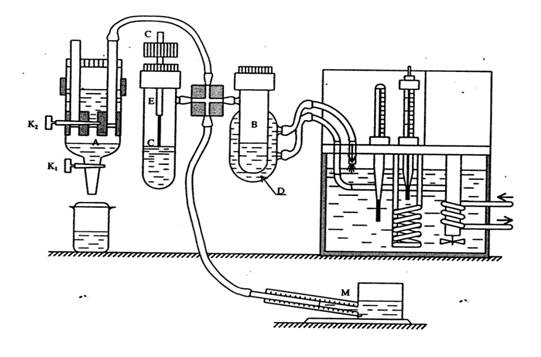
\includegraphics[scale=0.8]{image001_35.jpg}

    Ход работы:\\\\
    1)Убедимся в исправности установки\\\\
    2) Подберем частоту падения капель из аспиратора так, чтобы максимальное давление микроманометра не зависело от этой частоты. Для этого пузырьки не должны пробулькивать слишком часто (не чаще, чем $1$ пузырек в $5$ секунд)\\\\
    3) Измерим максимальное давление при пробулькивании пузырька (в спирте, при комнатной температуре $t = 21^{\circ}C$) и подсчитаем радиус капиляра. \\\\
    \begin{tabular}{c | c | c | c | c | c}
        $h$, дел. & $38$ & $39$ & $38$ & $39$ & $39$ \\ \hline
        $P$, Па & $74,3$ & $76,2$ & $74,3$ & $76,2$ & $76,2$ \\ 
    \end{tabular} \\\\
    $h$ - кол-во делений на микроманометре, $P$ - давление \\\\
    $P = c \cdot h \cdot \dfrac{\gamma_1}{\gamma_2} \cdot K \cdot 9.81$, где:\\
    \begin{itemize}
        \item $c$ = 1
        \item $K$ = 0.2 (коэффициент, зависящий от угла наклона)
        \item $\gamma_1 = 0.8066$ г/см$^3$~---~плотность залитого спирта
        \item $\gamma_2 = 0.8095$ г/см$^3$~---~плотность приборного спирта
    \end{itemize}
    $<P> = 75.4$ Па, $\sigma_p = \sqrt{\dfrac{1}{n(n-1)} \sum_{i=1}^n (P_i - <P>)^2} = 0.5$ Па $\rightarrow$ $<P> = 75.4 \pm 0.5$ Па \\\\
    4) Используя формулу Лапласа ($\Delta P = \dfrac{2 \sigma}{R}$) найдем радиус капиляра $R = \dfrac{2 \sigma}{<P>} = 0.59$ мм \\
    Сравним его с радиусом, измеренным с помощью микроскопа: $R_m = 0.6$ мм \\\\
    5) Перенесем (предварительно просушив) иглу в сосуд с водой. Измерим максимальное давление, когда игла лишь касается поверхности жидкости. \\\\
    \begin{tabular}{c | c | c | c | c | c}
        $h_1$, дел. & $101$ & $106$ & $107$ & $107$ & $108$ \\ \hline
        $P_1$, Па & $197.5$ & $207.2$ & $209.2$ & $209.2$ & $211.1$ \\
    \end{tabular} \\\\
    $<P_1> = 206.8 \pm 2.4$ Па\\\\
    6) Измерим $l_1 = 5.7$ см~---~расстояние от конца капиляра до некоторой части прибора.\\\\
    7) Утопим иглу до предела, но так, чтобы выходящие пузырьки не касались дна и снова измерим максимальное давление \\\\
    \begin{tabular}{c | c | c | c | c | c}
        $h_2$, дел. & $182$ & $182$ & $182$ & $182$ & $181$ \\ \hline
        $P_2$, Па & $355.8$ & $355.8$ & $355.8$ & $355.8$ & $353.8$ \\
    \end{tabular} \\\\
    $<P_2> = 355.4 \pm 0.4$ Па \\\\
    8) Снова измерим расстояние от конца капиляра до той же части прибора: $l_2 = 6.2$ см\\\\
    9) Подсчитаем $\Delta h = h_2 - h_1 = 1.5$ см. Сравним с $\Delta h'$, подсчитанным с помощью разницы давлений: $\Delta h' = \dfrac{<P_2> - <P_1>}{\rho g} = 1.5$ см \\\\
    10) Снимем зависимость $\sigma (t)$:\\\\
    \begin{tabular}{c | c | c | c | c | c | c | c}
        $t^{\circ}C$ & $27$ & $31$ & $35$ & $41$ & $45$ & $50$ & $55$\\ \hline
        $h,$ дел. & $180$ & $181$ & $177$ & $175$ & $172$ & $171$ & $168$\\ \hline
        $P_m,$ Па & $351.9$ & $353.8$ & $346.0$ & $342.1$ & $336.3$ & $334.3$ & $328.4$\\ \hline
        $\Delta P$, Па & $205.0$ & $207.0$ & $199.2$ & $195.3$ & $189.4$ & $187.4$ & $181.6$\\ \hline
        $\sigma$, Н/м & $0.062$ & $0.062$ & $0.060$ & $0.059$ & $0.057$ & $0.056$ & $0.054$\\ 
    \end{tabular} \\\\
    11) Методом наименьших квадратов вычисляем коэффициенты $k$ и $b$ в зависимости $\sigma = k \cdot t + b$: \\
    $k = (-2.7 \pm 0.2) \cdot 10^{-4}$ Н/м$^{\circ}$с; $b = (694 \pm 1) \cdot 10^{-4}$ Н/м \\\\
    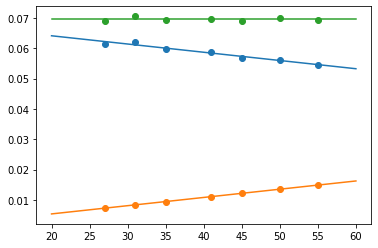
\includegraphics[scale=0.8]{загруженное.png}\\\\
    Зеленый график~---~$\dfrac{U}{F} = \sigma - t \cdot \dfrac{d \sigma}{dt} = \sigma - kT = b$ (поверхностная энергия единицы площади поверхности)\\
    Синий график~---~$\sigma = k \cdot t + b$ (коэффициент поверхностного натяжения от температуры) \\ 
    Оранжевый график~---~$q = -t \cdot \dfrac{d \sigma}{dt} = -k \cdot t$ \\\\
    12) Вывод: данный эксперимент с достаточно большой точностью позволяет выявить линейную зависимость коэффициента поверхностного натяжения от температуры.
\end{document}